\section{Nghiên Cứu Công Cụ Đại Diện B – Microsoft WinAppDriver}

\section{Nghiên Cứu Công Cụ: Microsoft WinAppDriver}
\subsection{Chuyên đề: Automation Testing cho Desktop Applications}

- \textbf{Người thực hiện:} Tùng (Tool B)
- \textbf{Mục tiêu báo cáo tuần:} Tổng quan công cụ, nguyên lý hoạt động, 3 năng lực cốt lõi (Record & Playback, Data-Driven, Checkpoints), ưu/nhược điểm và định hướng kịch bản demo đối trọng với Tool A (Katalon Studio).


\subsection{1. Tổng quan về Microsoft WinAppDriver}

\subsubsection{1.1 Thông tin chung}
* \textbf{Đơn vị phát triển:} Microsoft Corporation.
* \textbf{Mô hình bản quyền:} Mã nguồn mở (Open Source - Hoàn toàn miễn phí, không giới hạn tính năng hay thời gian sử dụng).
* \textbf{Chuẩn công nghệ:} Tuân thủ giao thức \textbf{W3C WebDriver} và chuẩn \textbf{Appium}.
* \textbf{Phạm vi hỗ trợ:} Kiểm thử tự động các ứng dụng chạy trên hệ điều hành Windows (UWP, WPF, WinForms, Win32).
* \textbf{Ngôn ngữ viết kịch bản:} Đa ngôn ngữ (C#/.NET, Python, Java, JavaScript/TypeScript...). Trong đó, \textbf{C#} và \textbf{Python} là hai ngôn ngữ phổ biến và tối ưu nhất.
* \textbf{Trường phái tiếp cận:} \textbf{Code-based / Developer-centric} (Kiểm thử thuần viết mã). Người kiểm thử làm việc trực tiếp trên các IDE tiêu chuẩn như Visual Studio, Rider hoặc VS Code.

\subsubsection{1.2 Lý do lựa chọn làm Tool B đối trọng với Tool A}
1. \textbf{Tạo ra sự đối lập rõ nét:} Nếu Katalon Studio đại diện cho trường phái \textit{All-in-one GUI Tool} (có giao diện bọc ngoài, hỗ trợ kéo thả / low-code), thì WinAppDriver đại diện cho trường phái \textit{Pure Code / SDK} (lập trình kiểm thử chuyên sâu cho Developer / SDET).
2. \textbf{Cùng chung nền tảng cốt lõi:} Cả hai công cụ đều sử dụng Windows UI Automation (UIA) để tương tác với ứng dụng. Điều này giúp việc so sánh giữa hai công cụ đạt tính khách quan tuyệt đối (chạy cùng đường đua, cùng case study).
3. \textbf{Chuẩn công nghiệp phổ biến:} Áp dụng cú pháp WebDriver quen thuộc (tương tự như Selenium trên Web và Appium trên Mobile), giúp người học dễ dàng kế thừa kỹ năng kiểm thử.


\subsection{2. Nguyên lý hoạt động trên Desktop App}

\subsubsection{2.1 Kiến trúc thực thi}
WinAppDriver hoạt động như một REST API Server độc lập đóng vai trò trung gian giữa kịch bản kiểm thử và hệ điều hành:

\begin{lstlisting}
┌──────────────────────────────────────────────┐
│  Test Script (C# / NUnit hoặc Python/pytest) │
│  - Dùng Appium / Selenium Client Library     │
└──────────────────────┬───────────────────────┘
                       │ HTTP / JSON Wire / W3C WebDriver (Port 4723)
                       ▼
┌──────────────────────────────────────────────┐
│  Microsoft WinAppDriver.exe                  │
│  (Lắng nghe tại 127.0.0.1:4723)             │
└──────────────────────┬───────────────────────┘
                       │ Native API Calls (C++ / COM)
                       ▼
┌──────────────────────────────────────────────┐
│  Windows UI Automation (UIA) Engine          │
└──────────────────────┬───────────────────────┘
                       │ Tương tác sự kiện hệ điều hành
                       ▼
┌──────────────────────────────────────────────┐
│  Application Under Test (AUT)                │
│  (WPF, WinForms, UWP, Win32)                 │
└──────────────────────────────────────────────┘
\end{lstlisting}


1. \textbf{Khởi tạo phiên (Session):} Kịch bản kiểm thử khởi tạo một \texttt{WindowsDriver} với các thông số cấu hình (\textit{DesiredCapabilities}) chỉ định đường dẫn ứng dụng (\texttt{app}), môi trường (\texttt{platformName: Windows}).
2. \textbf{Gửi lệnh WebDriver:} Các thao tác như tìm kiếm phần tử, click chuột, gửi phím được đóng gói thành các HTTP request gửi đến \texttt{http://127.0.0.1:4723}.
3. \textbf{Thông dịch UIA:} WinAppDriver tiếp nhận HTTP request và gọi trực tiếp các API của Windows UI Automation.
4. \textbf{Thực thi và phản hồi:} Windows thực thi thao tác trên ứng dụng đích và WinAppDriver đóng gói kết quả phản hồi (JSON) trả về cho Test Script.

\subsubsection{2.1.1 Cơ chế phân giải lệnh (Command Mapping) qua Port 4723}
* \textbf{Giao thức:} Client (C# NUnit) giao tiếp với WinAppDriver thông qua JSON Wire Protocol / W3C WebDriver specification bằng các HTTP Request chuẩn (POST, GET, DELETE).
* \textbf{Quá trình thực thi nội tại của WinAppDriver.exe:}
  1. Khi nhận lệnh \texttt{POST /session/{id}/element} kèm body \texttt{{"using": "name", "value": "ĐĂNG NHẬP"}}, WinAppDriver gọi hàm C++ của giao tiếp \texttt{IUIAutomation::CreatePropertyCondition(UIA_NamePropertyId, ...)} để duyệt cây UI Automation dựa trên tên hiển thị (Name) của control.
  2. Khi nhận lệnh click hoặc phím, nó gọi trực tiếp \texttt{IUIAutomationInvokePattern::Invoke()} hoặc \texttt{IUIAutomationValuePattern::SetValue()} của Windows OS, đảm bảo độ trễ gần như bằng 0 so với việc giả lập chuột ảo.

\subsubsection{2.2 Nhận diện phần tử giao diện (Object Recognition)}
Do WinAppDriver không có giao diện đồ họa riêng, việc định danh phần tử dựa trên các công cụ inspect độc lập của Microsoft:
* \textbf{Công cụ hỗ trợ inspect:}
  * \textbf{Accessibility Insights for Windows:} Công cụ hiện đại được Microsoft khuyến nghị, hỗ trợ kiểm tra cấu trúc cây giao diện và phát hiện nhanh các thuộc tính định danh.
  * \textbf{Inspect.exe:} Công cụ truyền thống đi kèm Windows SDK.
* \textbf{Cơ chế định vị trong mã nguồn:}
  * \texttt{AccessibilityId}: Trỏ trực tiếp vào thuộc tính \texttt{AutomationId} của control $\rightarrow$ \textbf{Phương thức định vị chuẩn và bền vững nhất}.
  * \texttt{Name}: Tìm theo nhãn hiển thị hoặc tiêu đề nút bấm.
  * \texttt{ClassName}: Tìm theo loại control (ví dụ: \texttt{TextBox}, \texttt{Button}).
  * \texttt{XPath}: Tìm theo đường dẫn phân cấp trong cây UI $\rightarrow$ Tốc độ tìm kiếm qua XPath trên WinAppDriver tương đối chậm, nên hạn chế dùng trừ khi không có ID.


\subsubsection{2.3 Quản lý Vòng đời Session (Session Lifecycle) với AppiumOptions}

Trong C# NUnit, vòng đời của một phiên kiểm thử tự động với WinAppDriver được quản lý chặt chẽ qua cấu trúc Setup - Test - TearDown:

\begin{lstlisting}
[TestFixture]
public class BaseTest
{
    protected WindowsDriver<WindowsElement> driver;
    private const string WinAppDriverUrl = "[http://127.0.0.1:4723](http://127.0.0.1:4723)";
    private const string AppPath = @"C:\Path\To\case-study-app\MiniSum\MiniSum.exe";

    [SetUp]
    public void InitializeSession()
    {
        AppiumOptions options = new AppiumOptions();
        options.AddAdditionalCapability("app", AppPath);
        options.AddAdditionalCapability("deviceName", "WindowsPC");
        options.AddAdditionalCapability("platformName", "Windows");
        
        // Khởi tạo phiên làm việc mới trên cổng 4723
        driver = new WindowsDriver<WindowsElement>(new Uri(WinAppDriverUrl), options);
        driver.Manage().Timeouts().ImplicitWait = TimeSpan.FromSeconds(3);
    }

    [TearDown]
    public void CleanupSession()
    {
        // Giải phóng tài nguyên và đóng ứng dụng sau khi chạy xong
        if (driver != null)
        {
            driver.CloseApp();
            driver.Quit();
            driver.Dispose();
        }
    }
}


---

## 3. Ba Năng Lực Cốt Lõi (Theo Lý Thuyết Kiểm Thử)

### 3.1 Record & Playback (Ghi & Phát lại kịch bản)
* **Thực trạng hỗ trợ:**
  * Bản thân WinAppDriver **không tích hợp sẵn trình Record & Playback** như Katalon Studio.
  * Lập trình viên kiểm thử chủ yếu dùng kỹ thuật *Inspect & Code*: Dùng công cụ inspect để lấy ID $\rightarrow$ Tự viết mã kịch bản.
  * *Mở rộng:* Có thể kết hợp với các công cụ ghi của bên thứ ba (như Appium Desktop Inspector) để ghi lại thao tác, nhưng mã sinh ra thường thô và phải cấu trúc lại.
* **Đánh giá:**
  * *Nhược điểm:* Tốc độ tạo kịch bản ban đầu chậm hơn so với việc bấm Record.
  * *Ưu điểm:* Kịch bản tự viết có cấu trúc rõ ràng, không chứa các thao tác rác hay độ trễ thừa, dễ áp dụng ngay các mẫu thiết kế chuẩn như **Page Object Model (POM)**.

### 3.2 Checkpoints & Assertions (Điểm kiểm tra kết quả)
* **Khái niệm:** Tự động hóa Test Oracle thông qua việc so khớp giữa kết quả thực tế lấy từ ứng dụng (`element.Text`, `element.Enabled`) với kết quả kỳ vọng.
* **Cơ chế thực hiện:**
  * WinAppDriver tận dụng trực tiếp các thư viện Assertion mạnh mẽ của ngôn ngữ lập trình (NUnit, xUnit, FluentAssertions đối với C#; hoặc pytest, unittest đối với Python).
  * *Ví dụ kiểm tra Text:* `Assert.AreEqual("Đăng nhập thành công", lblMessage.Text);`
  * *Ví dụ kiểm tra trạng thái:* `Assert.IsTrue(btnSubmit.Enabled);`
* **Xử lý chụp ảnh màn hình khi lỗi:**
  * Khi Assertion thất bại, framework cho phép bắt ngoại lệ và gọi hàm `driver.GetScreenshot().SaveAsFile(...)` để lưu bằng chứng lỗi phục vụ lập Bug Report.


\end{lstlisting}

[TearDown]
public void CaptureScreenOnFailure()
{
    // Kiểm tra trạng thái hoàn thành của Test Case
    var testStatus = TestContext.CurrentContext.Result.Outcome.Status;
    
    if (testStatus == NUnit.Framework.Interfaces.TestStatus.Failed)
    {
        string testName = TestContext.CurrentContext.Test.Name;
        string timestamp = DateTime.Now.ToString("yyyyMMdd_HHmmss");
        string directory = Path.Combine(AppDomain.CurrentDomain.BaseDirectory, "Screenshots");
        
        if (!Directory.Exists(directory))
            Directory.CreateDirectory(directory);

        string filePath = Path.Combine(directory, $"{testName}_FAIL_{timestamp}.png");

        // Chụp và lưu ảnh màn hình
        Screenshot screenshot = driver.GetScreenshot();
        screenshot.SaveAsFile(filePath, ScreenshotImageFormat.Png);
        
        // Đính kèm bằng chứng vào TestContext của NUnit
        TestContext.AddTestAttachment(filePath, "Screenshot khi kiểm thử thất bại");
    }

    driver?.Quit();
}




\subsubsection{3.3 Data-Driven Testing (Kiểm thử hướng dữ liệu)}
* \textbf{Cơ chế thực hiện:}
  \textit{ Tách rời hoàn toàn dữ liệu kiểm thử bằng cách tận dụng tính năng tham số hóa kịch bản (}Parameterized Testing*) của các Test Runner:
    * Trong \textbf{C# (NUnit):} Dùng thuộc tính \texttt{[TestCase]} cho dữ liệu nội tuyến hoặc \texttt{[TestCaseSource]} để đọc dữ liệu từ file Excel/CSV/JSON.
    * Trong \textbf{Python (pytest):} Dùng decorator \texttt{@pytest.mark.parametrize} kết hợp đọc file qua thư viện \texttt{pandas} hoặc \texttt{openpyxl}.
* \textbf{Ý nghĩa thực tế:}
  * Cho phép nạp trực tiếp danh sách \textbf{12 ca kiểm thử giá trị biên (BVA)} từ file Excel để chạy tự động qua cùng một kịch bản tính toán.
  * Dễ dàng tích hợp với các hệ thống quản trị cơ sở dữ liệu (SQL Server, MySQL) để kiểm thử các luồng dữ liệu lớn của doanh nghiệp.


\subsection{4. Đánh Giá Ưu Điểm \& Nhược Điểm}

\subsubsection{4.1 Ưu điểm}
1. \textbf{Miễn phí và mã nguồn mở 100\%:} Không chịu bất kỳ ràng buộc nào về chi phí bản quyền, số lượng máy chạy hay thời hạn dùng thử.
2. \textbf{Tuân thủ chuẩn W3C WebDriver:} Kỹ sư kiểm thử đã biết Selenium (Web) hoặc Appium (Mobile) có thể tiếp cận WinAppDriver gần như ngay lập tức mà không cần học một công cụ hoàn toàn mới.
3. \textbf{Tính linh hoạt và khả năng mở rộng vô hạn:}
   * Tự do lựa chọn cấu trúc dự án, áp dụng kiến trúc chuẩn như Page Object Model (POM) hoặc Screenplay.
   * Tự do tích hợp các thư viện xuất báo cáo chuyên nghiệp (Allure Report, ExtentReports, ReportPortal).
4. \textbf{Tối ưu cho quy trình DevOps & Git:} Mã kiểm thử là mã nguồn thuần (C#/Python), rất dễ kiểm soát phiên bản (VCS), giải quyết xung đột (conflict) và tích hợp vào pipeline CI/CD (GitHub Actions, Azure DevOps, Jenkins) thông qua lệnh build/test thông thường (\texttt{dotnet test} hoặc \texttt{pytest}).

\subsubsection{4.2 Nhược điểm \& Rào cản kỹ thuật}
1. \textbf{Trạng thái phát triển của dự án (Archive status):} Dự án WinAppDriver trên GitHub chính thức của Microsoft đã chuyển sang chế độ lưu trữ (archive/ngừng cập nhật tính năng mới từ năm 2023). Dù hiện tại vẫn chạy rất ổn định trên Windows 10/11, sự phát triển trong tương lai đang dần dịch chuyển sang dự án cộng đồng \textit{Appium Windows Driver}.
2. \textbf{Đòi hỏi kỹ năng lập trình:} Không có giao diện kéo thả hay chế độ Manual View; tester bắt buộc phải có tư duy phát triển phần mềm và thành thạo ngôn ngữ lập trình.
3. \textbf{Tốn thời gian xây dựng framework ban đầu:} Không có sẵn kho quản lý đối tượng (Object Repository) hay báo cáo tự động; nhóm phát triển phải tự tay viết code quản lý driver, cấu hình wait và cơ chế log/chụp màn hình.
4. \textbf{Phạm vi nền tảng hẹp:} Chỉ chạy trên hệ điều hành Windows, không hỗ trợ kiểm thử desktop trên macOS hay Linux.


\subsection{5. Định Hướng Kịch Bản Demo Cho Nhóm (Dùng Chung Case Study Với Tool A)}

Để đảm bảo tính đối chiếu công bằng với Katalon Studio, kịch bản của WinAppDriver sẽ thực hiện trên \textbf{cùng ứng dụng mẫu} và \textbf{cùng bộ dữ liệu}:

\begin{lstlisting}
[Demo 1: Thiết lập] ──► [Demo 2: Cơ bản] ──► [Demo 3: Nâng cao]
 Khởi động driver        Viết code Test Case   Data-Driven BVA
 Soi ID bằng UIA         Assertion + Chụp ảnh  Đọc file Excel
\end{lstlisting}


\subsubsection{5.1 Demo 1: Cài đặt và chuẩn bị môi trường}
* \textbf{Mục tiêu:} Chứng minh cấu hình môi trường chuẩn mã nguồn mở.
* \textbf{Các bước chính:}
  1. Khởi chạy \texttt{WinAppDriver.exe} ở quyền Administrator (lắng nghe tại cổng 4723).
  2. Mở công cụ \textit{Accessibility Insights for Windows} để bóc tách các \texttt{AutomationId} trên ứng dụng mẫu.
  3. Mở Visual Studio (hoặc VS Code), tạo dự án kiểm thử với thư viện \texttt{Appium.WebDriver} và \texttt{NUnit}.

\subsubsection{5.2 Demo 2: Kịch bản cơ bản (Code-based + Checkpoint Assertion)}
* \textbf{Mục tiêu:} Minh họa cách viết kịch bản kiểm thử chuẩn cấu trúc bằng mã nguồn (Chức năng Đăng nhập).
* \textbf{Các bước chính:}
  1. Khởi tạo phiên làm việc với ứng dụng qua \texttt{WindowsDriver<WindowsElement>}.
  2. Dùng lệnh \texttt{FindElementByAccessibilityId} để nhập tài khoản, mật khẩu và click nút Submit.
  3. Áp dụng Checkpoint bằng câu lệnh \texttt{Assert.AreEqual("Đăng nhập thành công", lblMessage.Text)}.
  4. Cố tình gây lỗi để minh họa cơ chế tự động chụp ảnh màn hình lưu vào thư mục dự án khi kiểm thử thất bại.

\subsubsection{5.3 Demo 3: Kịch bản nâng cao (Data-Driven BVA với File Excel)}
* \textbf{Mục tiêu:} Chứng minh năng lực kiểm thử dữ liệu lớn kết hợp kỹ thuật phân tích giá trị biên.
* \textbf{Các bước chính:}
  1. Sử dụng thư viện đọc Excel để nạp bộ dữ liệu \textbf{12 ca biên BVA} của bài toán tính tổng 2 số nguyên.
  2. Tham số hóa phương thức kiểm thử với \texttt{[TestCaseSource]}.
  3. Thực thi tự động 12 ca kiểm thử liên tiếp bằng lệnh \texttt{dotnet test}.
  4. Xem báo cáo kết quả thực thi chi tiết dạng XML/HTML qua công cụ Test Explorer.


\subsection{6. Khi Nào Nên \& Không Nên Chọn WinAppDriver}

\begin{table}[H]
\centering
\begin{tabular}{|l|l|}
\hline
\textbf{Nên chọn Microsoft WinAppDriver} & \textbf{Khi nào nên cân nhắc công cụ khác (như Katalon Studio)} \\ \hline
Đội ngũ kiểm thử là các kỹ sư SDET hoặc lập trình viên có kỹ năng viết code tốt. & Đội ngũ có nhiều Manual Tester, cần giao diện đồ họa và tính năng Record \& Playback để làm quen nhanh. \\ \hline
Muốn tự do hoàn toàn trong việc thiết kế framework kiểm thử (áp dụng POM, Screenplay). & Cần một giải pháp trọn gói (All-in-one) có sẵn Object Repository và hệ thống báo cáo hoàn chỉnh ngay khi cài đặt. \\ \hline
Dự án yêu cầu 100\% phần mềm mã nguồn mở, không có ngân sách mua license thương mại. & Cần một công cụ đang được nhà sản xuất cam kết hỗ trợ kỹ thuật dài hạn và cập nhật tính năng mới liên tục. \\ \hline
Muốn tích hợp sâu vào quy trình CI/CD nội bộ của nhóm phát triển phần mềm qua Git. & Dự án cần triển khai gấp trong thời gian ngắn mà không có thời gian lập trình khung framework. \\ \hline
\end{tabular}
\end{table}




\subsection{7. Thực Nghiệm Kịch Bản Demo và Minh Chứng Kết Quả}

\subsubsection{7.1 Khởi động dịch vụ WinAppDriver}
Quá trình kiểm thử bắt đầu bằng việc khởi chạy tiến trình \texttt{WinAppDriver.exe} dưới quyền quản trị (Administrator), sẵn sàng lắng nghe các lệnh HTTP RESTful tại cổng mặc định \texttt{4723}.

\begin{figure}[H]
\centering
% 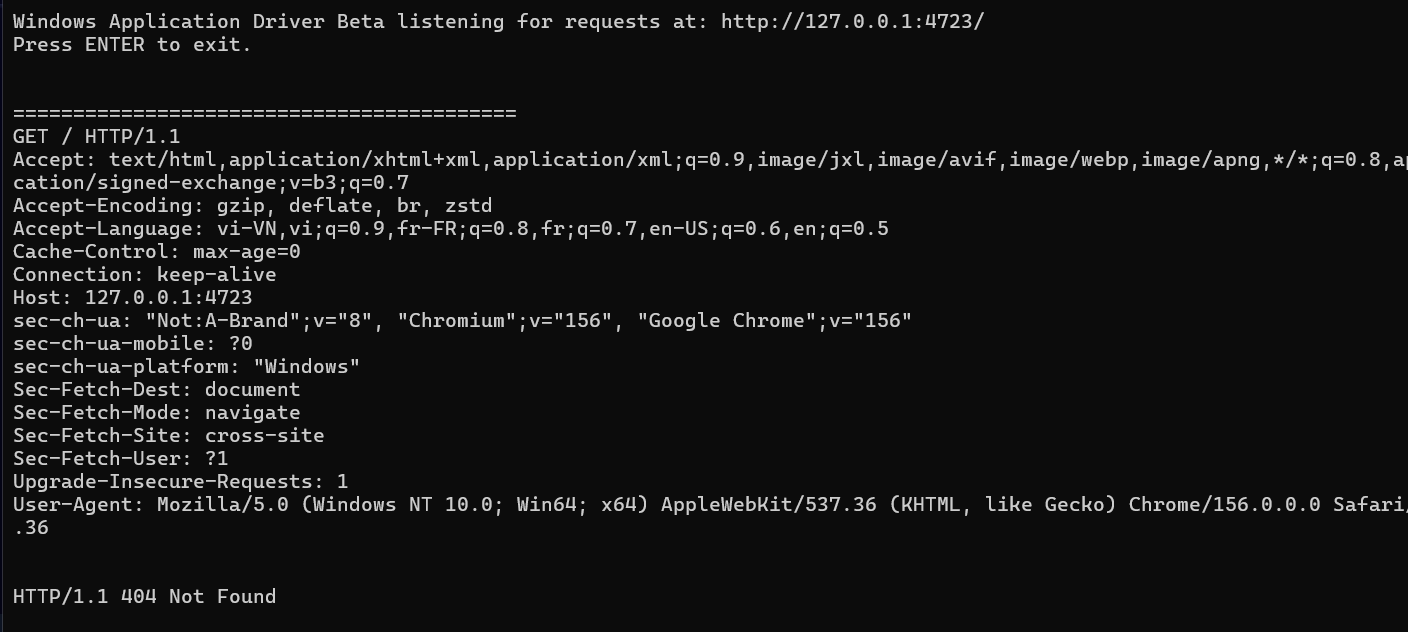
\includegraphics[width=0.85\textwidth]{../demo-scripts/winappdriver/screen short/winappdriver.png}
\caption{Cửa sổ Console khởi chạy WinAppDriver}
\end{figure}


\subsubsection{7.2 Khảo sát phần tử giao diện bằng Accessibility Insights for Windows}
Nhóm sử dụng công cụ \textit{Accessibility Insights for Windows} để bóc tách cây giao diện UI Automation (UIA) và trích xuất các thuộc tính định danh \texttt{AutomationId} đáng tin cậy của ứng dụng \texttt{MiniSum.exe}:

\begin{figure}[H]
\centering
% 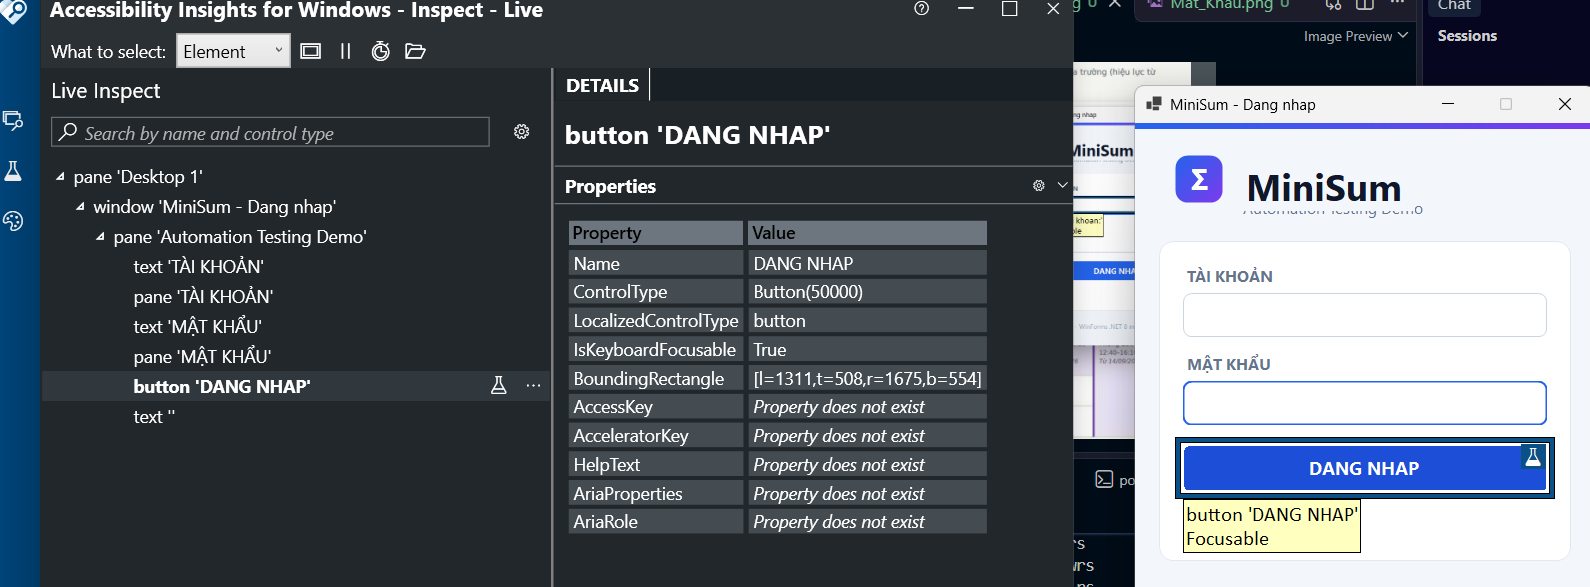
\includegraphics[width=0.85\textwidth]{../demo-scripts/winappdriver/screen short/DANG_NHAP.png}
\caption{Accessibility Insights - Màn hình Đăng nhập}
\end{figure}


\begin{figure}[H]
\centering
% 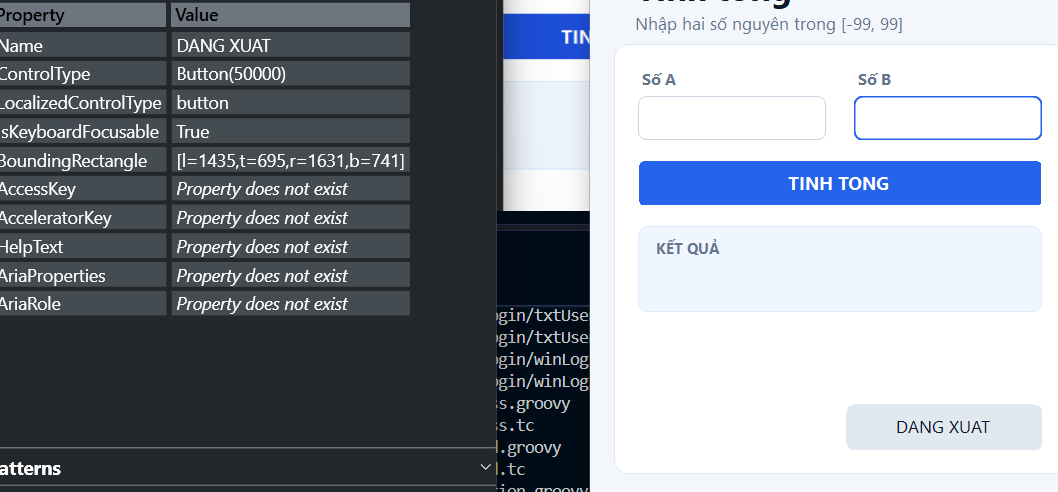
\includegraphics[width=0.85\textwidth]{../demo-scripts/winappdriver/screen short/DANG_XUAT.png}
\caption{Accessibility Insights - Nút Đăng xuất}
\end{figure}


\begin{figure}[H]
\centering
% 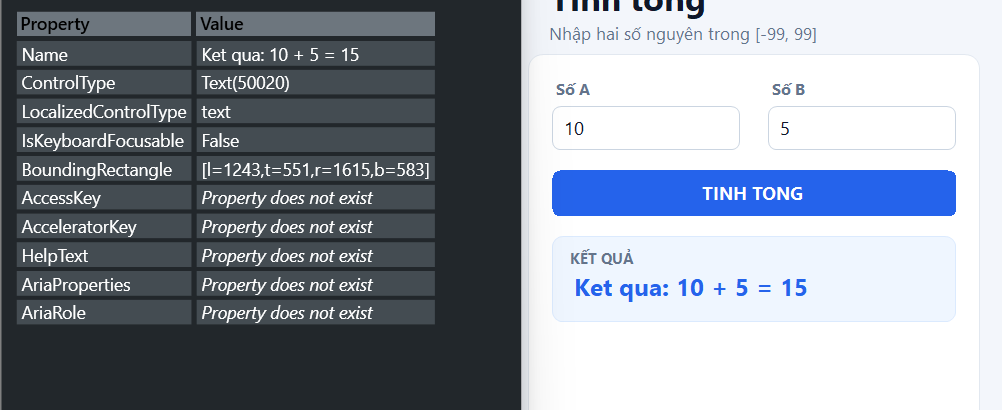
\includegraphics[width=0.85\textwidth]{../demo-scripts/winappdriver/screen short/ketqua.png}
\caption{Accessibility Insights - Ô hiển thị kết quả}
\end{figure}


\begin{figure}[H]
\centering
% 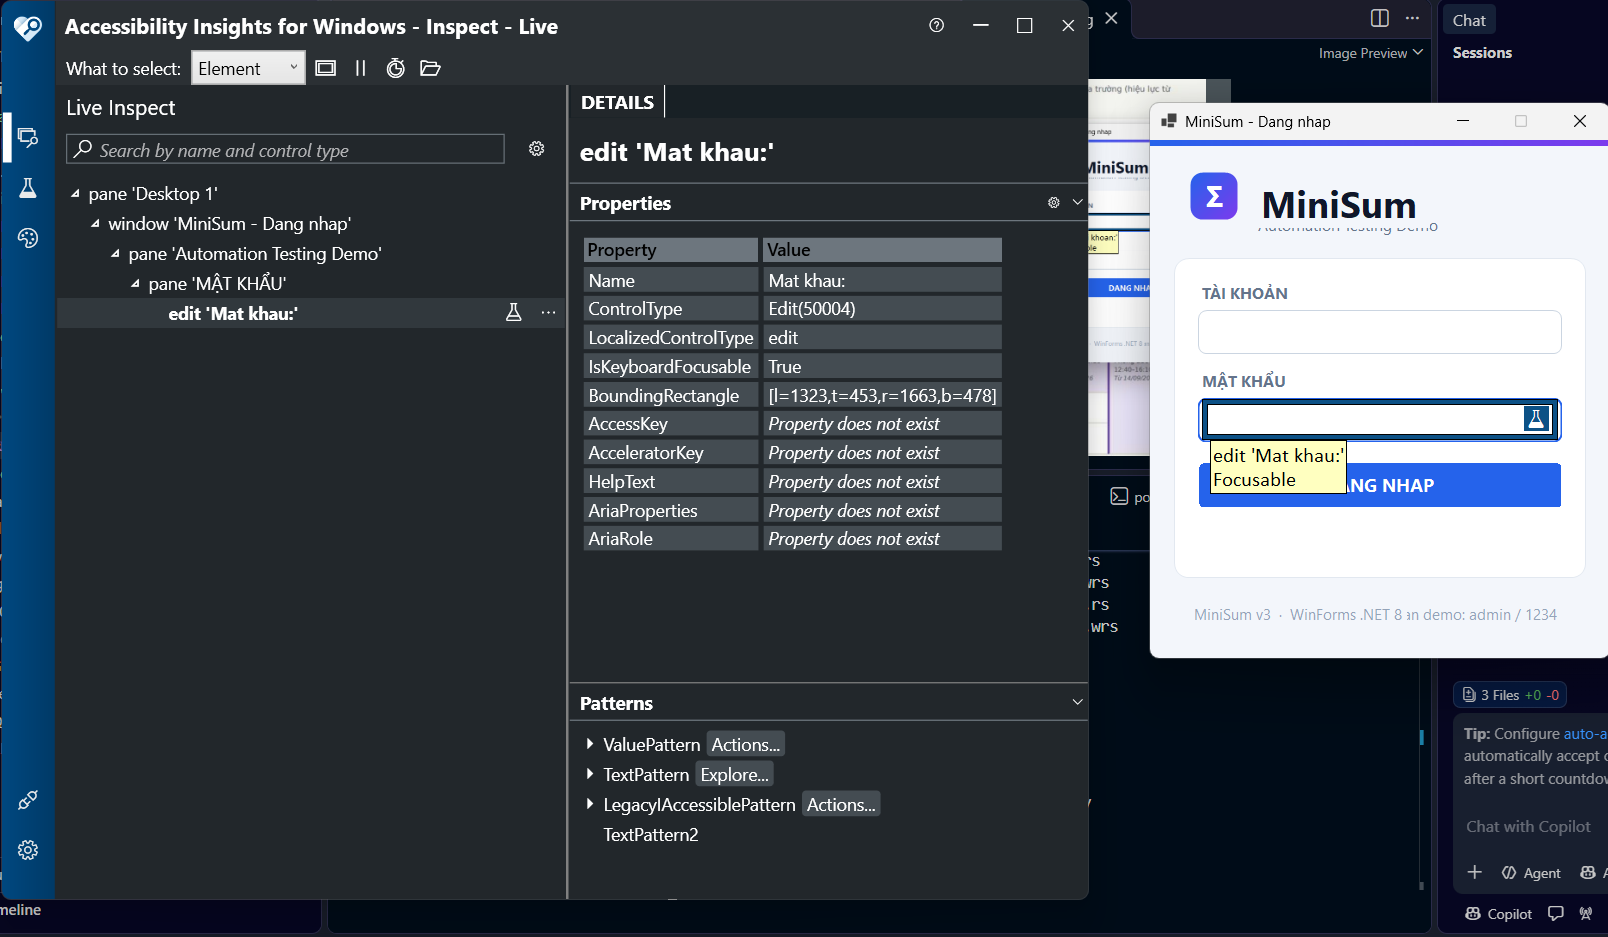
\includegraphics[width=0.85\textwidth]{../demo-scripts/winappdriver/screen short/Mat_Khau.png}
\caption{Accessibility Insights - Trường nhập Mật khẩu}
\end{figure}


\begin{figure}[H]
\centering
% 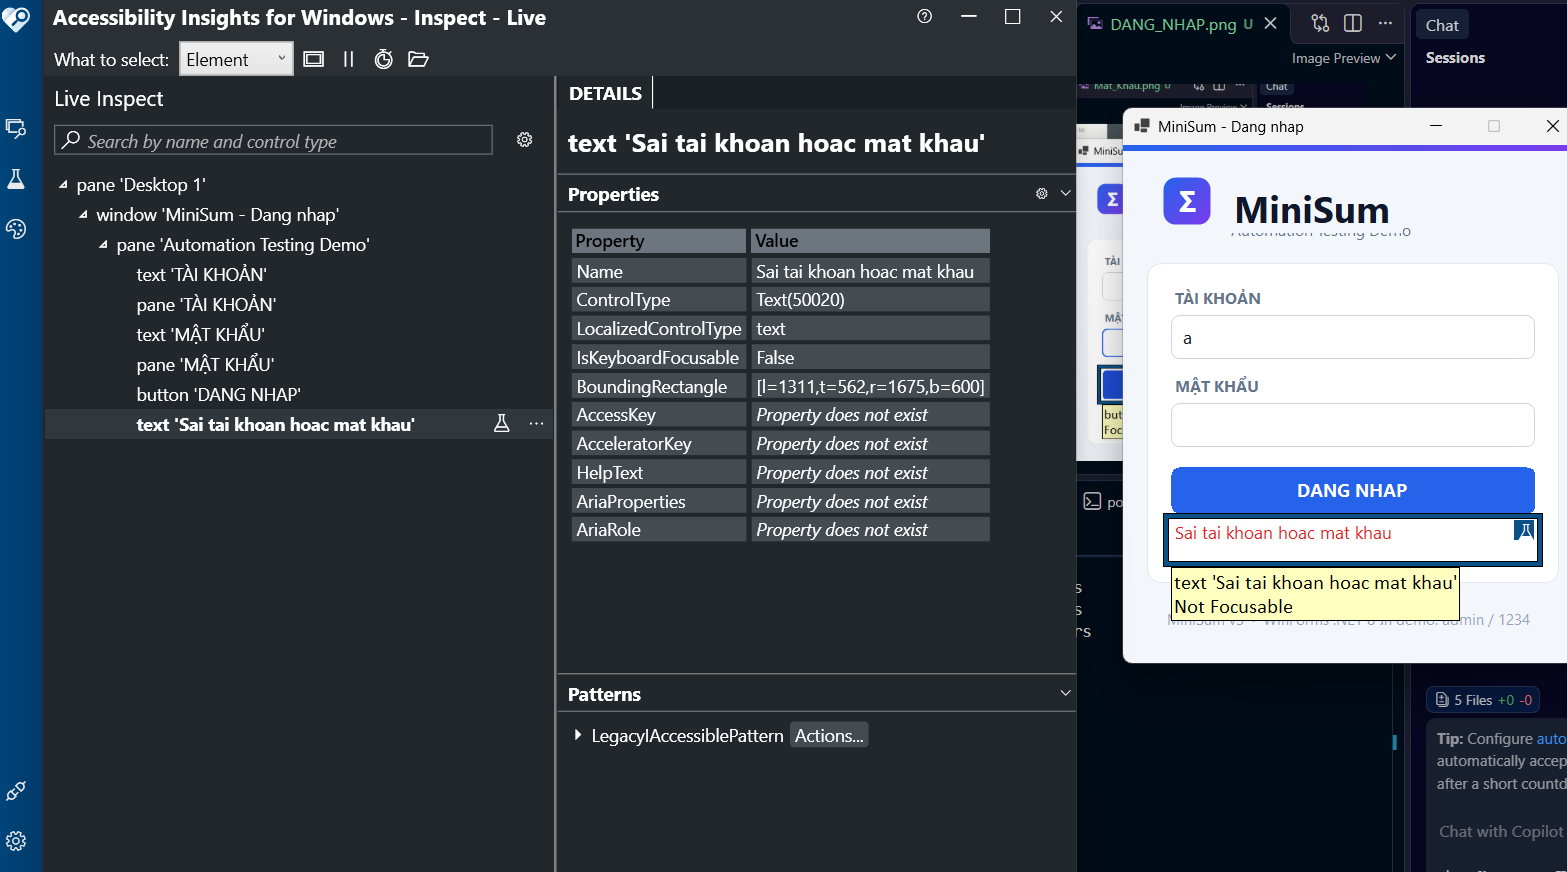
\includegraphics[width=0.85\textwidth]{../demo-scripts/winappdriver/screen short/Sai_tai_khoan_hoac_mat_khau.png}
\caption{Accessibility Insights - Thông báo sai đăng nhập}
\end{figure}


\begin{figure}[H]
\centering
% 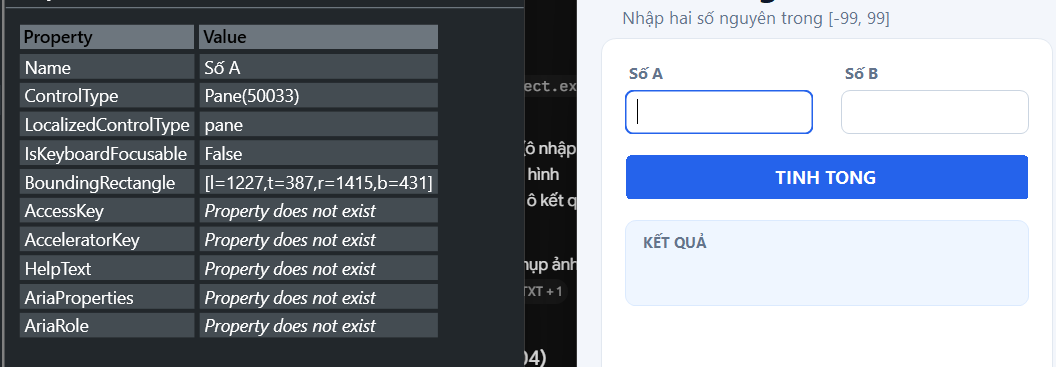
\includegraphics[width=0.85\textwidth]{../demo-scripts/winappdriver/screen short/So_A.png}
\caption{Accessibility Insights - Ô nhập số A}
\end{figure}


\begin{figure}[H]
\centering
% 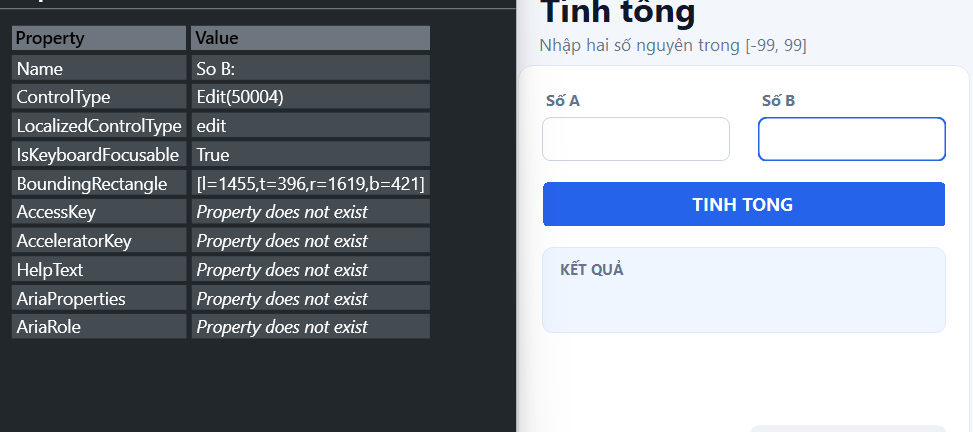
\includegraphics[width=0.85\textwidth]{../demo-scripts/winappdriver/screen short/So_B.png}
\caption{Accessibility Insights - Ô nhập số B}
\end{figure}


\begin{figure}[H]
\centering
% 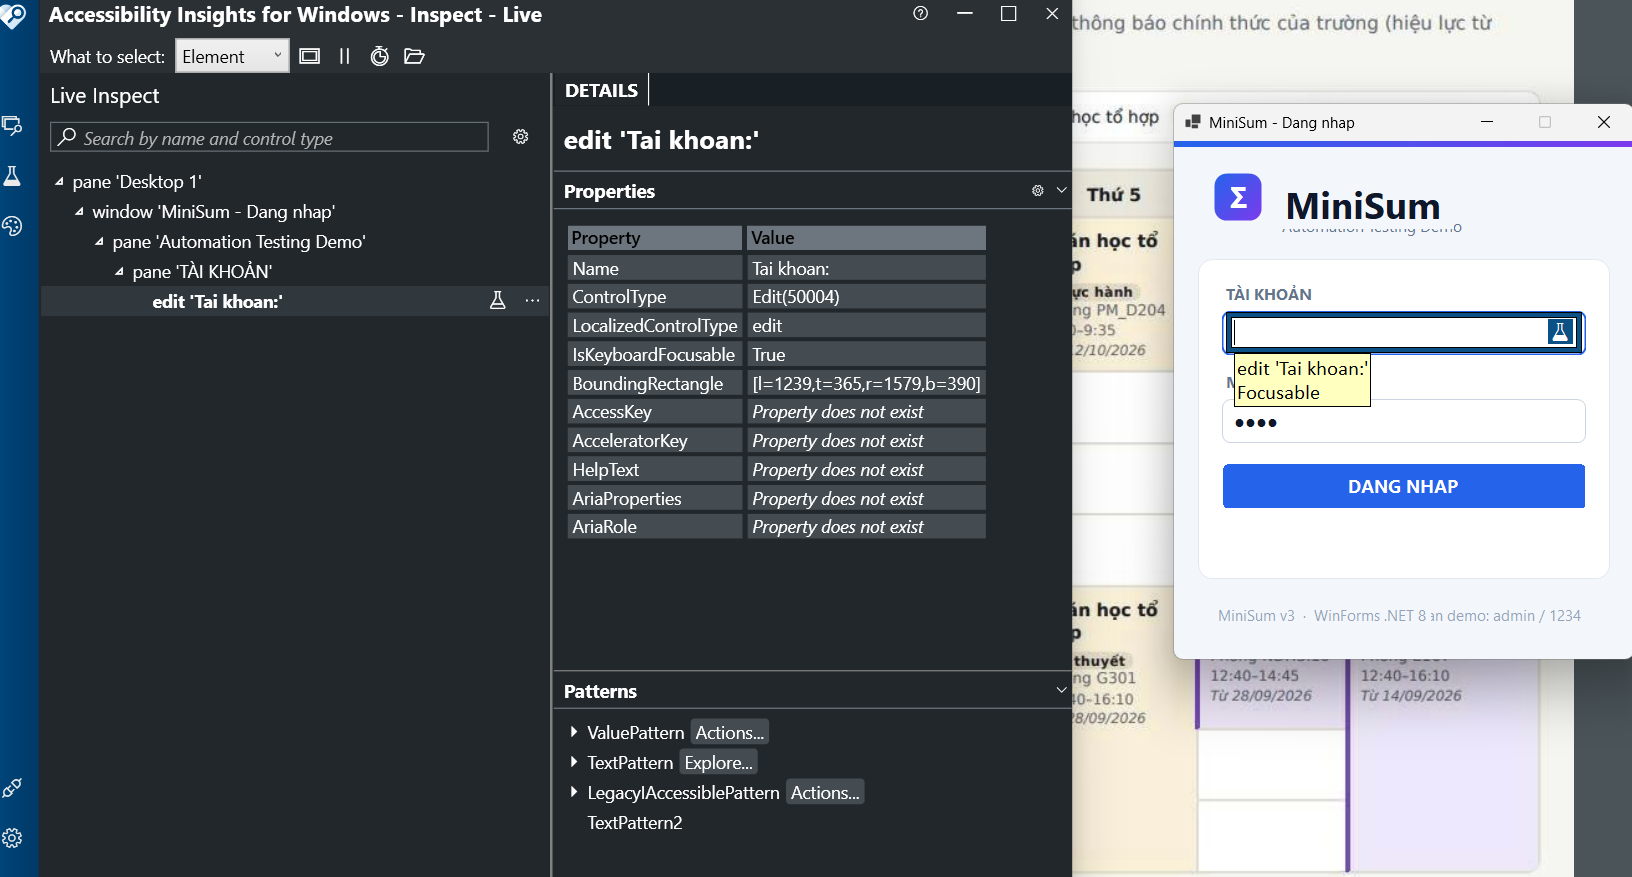
\includegraphics[width=0.85\textwidth]{../demo-scripts/winappdriver/screen short/Tai_Khoan.png}
\caption{Accessibility Insights - Trường tài khoản}
\end{figure}


\begin{figure}[H]
\centering
% 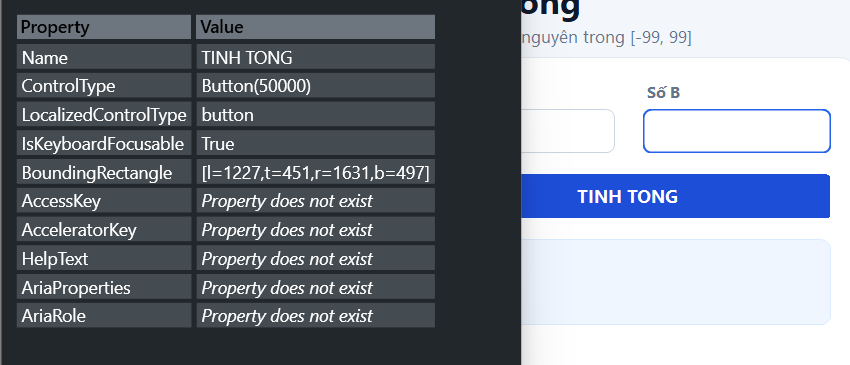
\includegraphics[width=0.85\textwidth]{../demo-scripts/winappdriver/screen short/Tinh_Tong.png}
\caption{Accessibility Insights - Nút Tính tổng}
\end{figure}


\subsubsection{7.3 Kết quả thực thi kiểm thử trên Terminal}
Sau khi xây dựng hoàn tất mã nguồn kiểm thử NUnit theo mô hình Page Object Model (POM), kịch bản được thực thi hoàn toàn tự động thông qua dòng lệnh \texttt{dotnet test}.

\begin{figure}[H]
\centering
% 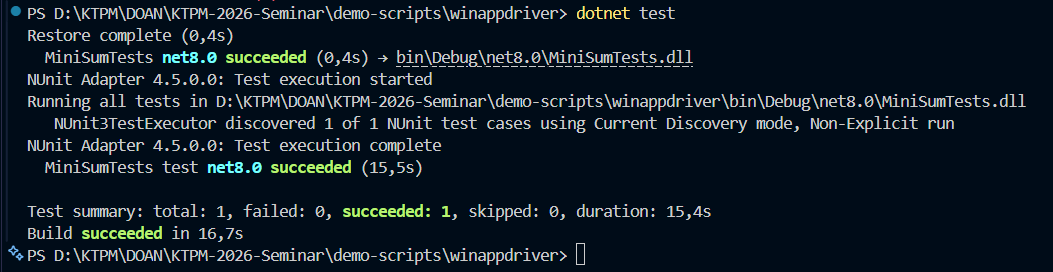
\includegraphics[width=0.85\textwidth]{../demo-scripts/winappdriver/screen short/test_pass_terminal.png}
\caption{Kết quả thực thi Test Pass trên Terminal}
\end{figure}


\begin{figure}[H]
\centering
% 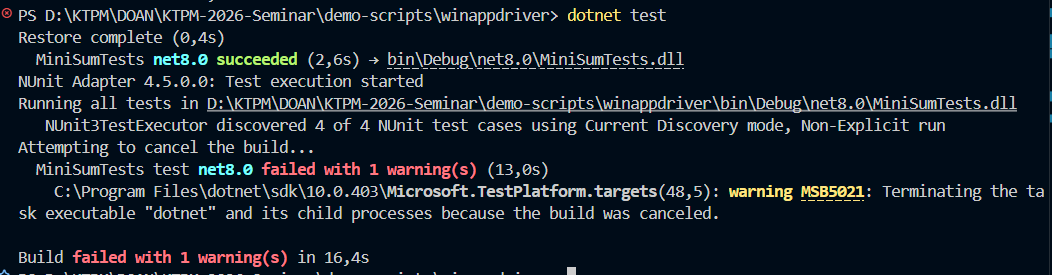
\includegraphics[width=0.85\textwidth]{../demo-scripts/winappdriver/screen short/image.png}
\caption{Cơ chế bẫy lỗi và chụp ảnh tự động khi test fail}
\end{figure}

